\documentclass[11pt,a4paper]{article}

\usepackage{fontspec}
\setmonofont{DejaVuSansMono.ttf}[Scale=0.85,BoldFont=DejaVuSansMono-Bold.ttf,ItalicFont=DejaVuSansMono-Oblique.ttf]
\usepackage{amsmath,amssymb,amsthm}
\usepackage{mathtools}
\usepackage[margin=1.15in]{geometry}
\usepackage{microtype}
\usepackage{tikz}
\usetikzlibrary{arrows.meta,calc,decorations.pathreplacing}
\usepackage{listings}
\usepackage{xcolor}
\usepackage[numbers,sort&compress]{natbib}
\usepackage[hidelinks]{hyperref}
\usepackage{url}
\usepackage{caption}

\definecolor{leankw}{HTML}{1F4E9E}
\definecolor{leancomment}{HTML}{5B6B5B}
\lstdefinelanguage{lean}{
  morekeywords={theorem,def,structure,where,by,fun,open,namespace,end,noncomputable,section,
    variable,import,rintro,exact,rw,constructor,refine,obtain,have,simp,linarith,rfl,example},
  sensitive=true,
  morecomment=[l]{--},
  morecomment=[s]{/-}{-/},
}
\lstset{
  language=lean,
  basicstyle=\ttfamily\small,
  keywordstyle=\color{leankw}\bfseries,
  commentstyle=\color{leancomment}\itshape,
  columns=fullflexible,
  keepspaces=true,
  frame=single,
  rulecolor=\color{black!25},
  xleftmargin=1em,
  xrightmargin=1em,
  aboveskip=1em,
  belowskip=1em,
}

\newtheorem{theorem}{Theorem}
\newtheorem{proposition}[theorem]{Proposition}
\newtheorem{lemma}[theorem]{Lemma}
\newtheorem{corollary}[theorem]{Corollary}
\theoremstyle{definition}
\newtheorem{definition}[theorem]{Definition}
\theoremstyle{remark}
\newtheorem{remark}[theorem]{Remark}
\newtheorem{example}[theorem]{Example}

\newcommand{\R}{\mathbb{R}}
\newcommand{\C}{\mathbb{C}}
\newcommand{\Disc}{\mathbb{D}}
\newcommand{\RR}{\mathcal{R}}
\newcommand{\Core}{\mathcal{K}}
\newcommand{\abs}[1]{\left\lvert #1 \right\rvert}
\newcommand{\norm}[1]{\left\lVert #1 \right\rVert}
\DeclareMathOperator{\dist}{dist}
\DeclareMathOperator{\Re_}{Re}
\DeclareMathOperator{\Im_}{Im}

\title{\textbf{On the Corner Radii of Nested Rounded Rectangles}\\[0.4em]
\large A Machine-Checked Proof of the Law $R = r + d$}
\author{Steve Ruiz}
\date{November 2026}

\begin{document}
\maketitle

\begin{abstract}
When a rounded rectangle of corner radius $r$ is placed inside a larger rounded rectangle with a
uniform gap of width $d$ on all sides, the outer corner radius must be $R = r + d$. This
relation is known to every practitioner of graphical user-interface design, is encoded in the
corner-shaping rules of the CSS Backgrounds and Borders specification, and is violated with some
regularity in production software. We give a precise statement of the law in the Euclidean plane,
prove that the closed $d$-neighbourhood of a rounded rectangle of radius $r$ is a rounded
rectangle of radius $r + d$, and prove that no other radius produces a uniform gap. We further
show that the common practice of assigning both shapes the same radius yields a uniform gap only
in the degenerate case $d = 0$, and that an outer radius smaller than the gap is not realisable by
any inner shape. All results are formalized in the Lean~4 theorem prover against the Mathlib
library, and depend on no axioms beyond the three standard ones.
\end{abstract}

\section{Introduction}

Consider a card with rounded corners resting inside a container, also with rounded corners,
separated from it by a constant padding $d$. A recurring question in interface design is which
corner radius to give the container. Two answers are in circulation. The first assigns the same
radius to both shapes. The second, which we shall call the \emph{nested radius law}, prescribes
\begin{equation}\label{eq:law}
  R = r + d,
\end{equation}
where $r$ is the radius of the inner shape and $R$ that of the outer. The visual consequence of the
first answer is familiar: the gap between the two shapes, constant along the straight edges,
swells at the corners (Figure~\ref{fig:nested}).

The law \eqref{eq:law} is a special case of a classical fact about parallel bodies: the outer
parallel body at distance $d$ of the outer parallel body at distance $r$ of a set $K$ is the outer
parallel body at distance $r + d$ of $K$~\citep{steiner1840,minkowski1903,hadwiger1957,schneider2014}.
In the language of mathematical morphology, dilation by a disc of radius $r$ followed by dilation
by a disc of radius $d$ is dilation by a disc of radius $r +
d$~\citep{matheron1975,serra1982}. The same observation underlies offsetting in solid modelling and
the theory of offset curves~\citep{rossignac1986,maekawa1999}. In the web platform, the CSS
Backgrounds and Borders specification states the inverse form of the law: the radius of the
padding edge is the radius of the border edge less the border width, clamped at
zero~\citep{css3backgrounds}.

Despite this pedigree, we are not aware of a machine-checked proof. Recent years have seen
proof assistants, often with the help of large language models, applied to problems of
considerable depth. The present work addresses a problem of considerably less depth, in the
belief that a result consulted this often deserves the same standard of rigour. Our contributions
are:
\begin{enumerate}
  \item a precise definition of the rounded rectangle and of the \emph{uniform gap} relation
        between two planar sets (Section~\ref{sec:defs});
  \item a proof that the uniform-gap outer shape of a rounded rectangle exists, is a rounded
        rectangle, and has radius $r + d$ (Theorem~\ref{thm:offset});
  \item a proof that a rounded rectangle determines its parameters, from which it follows that
        $r + d$ is the \emph{only} admissible outer radius (Theorems~\ref{thm:inj}
        and~\ref{thm:main});
  \item corollaries addressing the equal-radius practice and the case $R < d$
        (Section~\ref{sec:corollaries}); and
  \item a complete formalization in Lean~4~\citep{lean4} using Mathlib~\citep{mathlib2020}
        (Section~\ref{sec:lean}).
\end{enumerate}

\begin{figure}[t]
\centering
\resizebox{\linewidth}{!}{%
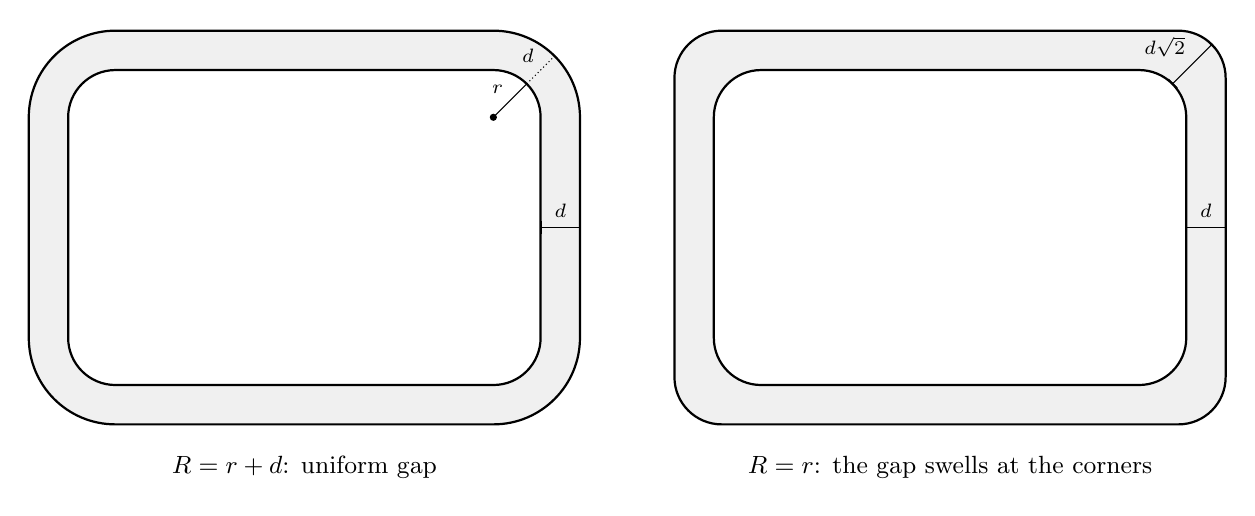
\begin{tikzpicture}
  % Left panel: correct
  \begin{scope}
    \fill[black!6, rounded corners=1.1cm] (-3.5,-2.5) rectangle (3.5,2.5);
    \draw[thick, rounded corners=1.1cm] (-3.5,-2.5) rectangle (3.5,2.5);
    \fill[white, rounded corners=0.6cm] (-3,-2) rectangle (3,2);
    \draw[thick, rounded corners=0.6cm] (-3,-2) rectangle (3,2);
    \fill (2.4,1.4) circle (1.3pt);
    \draw[thin] (2.4,1.4) -- (2.824,1.824)
      node[midway, above left=-1pt, font=\scriptsize] {$r$};
    \draw[thin, densely dotted] (2.824,1.824) -- (3.178,2.178)
      node[midway, above left=-1pt, font=\scriptsize] {$d$};
    \node[font=\small] at (0,-3.05) {$R = r + d$: uniform gap};
    \draw[|-|, thin] (3.0,0) -- (3.5,0) node[midway, above, font=\scriptsize] {$d$};
  \end{scope}
  % Right panel: equal radii
  \begin{scope}[xshift=8.2cm]
    \fill[black!6, rounded corners=0.6cm] (-3.5,-2.5) rectangle (3.5,2.5);
    \draw[thick, rounded corners=0.6cm] (-3.5,-2.5) rectangle (3.5,2.5);
    \fill[white, rounded corners=0.6cm] (-3,-2) rectangle (3,2);
    \draw[thick, rounded corners=0.6cm] (-3,-2) rectangle (3,2);
    \draw[|-|, thin] (3.0,0) -- (3.5,0) node[midway, above, font=\scriptsize] {$d$};
    \draw[|-|, thin] (2.824,1.824) -- (3.324,2.324)
      node[midway, above left=-1pt, font=\scriptsize] {$d\sqrt2$};
    \node[font=\small] at (0,-3.05) {$R = r$: the gap swells at the corners};
  \end{scope}
\end{tikzpicture}%
}
\caption{Left: an inner rounded rectangle of radius $r$ and the outer rounded rectangle of radius
$r + d$ (Theorem~\ref{thm:offset}). Both top-right corner arcs share the marked centre, and their
radii differ by $d$. Right: with equal radii, the gap measured along the
diagonal at each corner is $d\sqrt{2}$ rather than $d$ (Proposition~\ref{prop:swell}).}
\label{fig:nested}
\end{figure}

\section{Definitions}\label{sec:defs}

We identify the Euclidean plane with $\C$, writing $z = x + iy$ and
$\norm{z} = \sqrt{x^2 + y^2}$. For $A, B \subseteq \C$ the \emph{Minkowski sum} is
$A + B = \{a + b : a \in A,\ b \in B\}$. We write $\Disc_\rho = \{z : \norm{z} \le \rho\}$ for the
closed disc of radius $\rho \ge 0$ about the origin, and, for $S \subseteq \C$ and $d \ge 0$,
\[
  S^{(d)} = \{ z \in \C : \dist(z, S) \le d \}
\]
for the closed $d$-neighbourhood (outer parallel set) of $S$, where
$\dist(z, S) = \inf_{s \in S} \norm{z - s}$.

\begin{definition}[Rounded rectangle]\label{def:rr}
Let $a, b, r \in \R$. The \emph{core} with parameters $(a, b, r)$ is the closed rectangle
\[
  \Core(a, b, r) = \{ z \in \C : \abs{\Re_ z} \le a - r,\ \abs{\Im_ z} \le b - r \},
\]
and the \emph{rounded rectangle} with half-width $a$, half-height $b$ and corner radius $r$ is
\[
  \RR(a, b, r) = \Core(a, b, r) + \Disc_r .
\]
The parameters are \emph{admissible} if $0 \le r \le \min(a, b)$.
\end{definition}

For admissible parameters, $\RR(a, b, r)$ is the familiar shape: its bounding box is
$[-a, a] \times [-b, b]$, its edges are straight, and its four corners are circular arcs of
radius $r$ centred at the vertices $(\pm(a - r), \pm(b - r))$ of the core. The cases $r = 0$
(a rectangle) and $r = a = b$ (a disc) are included.

\begin{definition}[Uniform gap]\label{def:gap}
Let $d \ge 0$. A set $O \subseteq \C$ \emph{surrounds} a set $I \subseteq \C$ \emph{with uniform
gap} $d$ if $O = I^{(d)}$.
\end{definition}

Definition~\ref{def:gap} says that $O$ contains exactly those points lying within distance $d$ of
$I$. For compact $I$ this is equivalent to $O = I + \Disc_d$; we use both forms below.

\begin{remark}[Choice of norm]
The identification of the plane with $\C$ rather than with $\R \times \R$ is deliberate. In
Mathlib the product $\R \times \R$ carries the supremum norm, under which every ``disc'' is a
square, every rounded rectangle is a rectangle, and the questions considered here are vacuous.
\end{remark}

\section{Existence}\label{sec:existence}

\begin{lemma}\label{lem:disc}
For $\rho, \sigma \ge 0$, $\Disc_\rho + \Disc_\sigma = \Disc_{\rho + \sigma}$.
\end{lemma}

\begin{proof}
The inclusion $\subseteq$ is the triangle inequality. Conversely, given $\norm{z} \le \rho +
\sigma$ with $z \ne 0$, write $z = \frac{\rho}{\rho + \sigma} z + \frac{\sigma}{\rho + \sigma} z$;
the case $z = 0$ or $\rho + \sigma = 0$ is immediate.
\end{proof}

\begin{lemma}\label{lem:compact}
For compact $S \subseteq \C$ and $d \ge 0$, $S^{(d)} = S + \Disc_d$.
\end{lemma}

\begin{proof}
If $\dist(z, S) \le d$, the infimum is attained at some $s \in S$ by compactness, and
$z = s + (z - s)$ with $\norm{z - s} \le d$. The converse is immediate.
\end{proof}

\begin{theorem}[Offset theorem]\label{thm:offset}
Let $r, d \ge 0$ and $a, b \in \R$. Then
\[
  \RR(a, b, r)^{(d)} = \RR(a + d,\ b + d,\ r + d).
\]
If $(a, b, r)$ is admissible, so is $(a + d, b + d, r + d)$.
\end{theorem}

\begin{proof}
$\RR(a, b, r)$ is the sum of two compact sets and hence compact. Observe that
$\Core(a + d, b + d, r + d) = \Core(a, b, r)$, since $(a + d) - (r + d) = a - r$ and likewise for
$b$. By Lemma~\ref{lem:compact}, associativity of Minkowski addition, and Lemma~\ref{lem:disc},
\[
  \RR(a, b, r)^{(d)}
  = \bigl(\Core(a, b, r) + \Disc_r\bigr) + \Disc_d
  = \Core(a, b, r) + \Disc_{r + d}
  = \RR(a + d, b + d, r + d).
\]
Admissibility is preserved because $r + d \ge 0$ and $r + d \le a + d$, $r + d \le b + d$.
\end{proof}

\section{Uniqueness}\label{sec:uniqueness}

Theorem~\ref{thm:offset} shows that $r + d$ \emph{suffices}. To conclude that it is
\emph{necessary}, we show that a rounded rectangle, as a subset of the plane, determines its three
parameters.

\begin{lemma}\label{lem:bounds}
Let $z \in \RR(a, b, r)$. Then $\abs{\Re_ z} \le a$ and $\abs{\Im_ z} \le b$. If $(a, b, r)$ is
admissible, then $a$ and $ib$ belong to $\RR(a, b, r)$.
\end{lemma}

\begin{proof}
Write $z = k + v$ with $k \in \Core(a, b, r)$ and $\norm{v} \le r$. Then
$\abs{\Re_ z} \le \abs{\Re_ k} + \abs{\Re_ v} \le (a - r) + r$, and similarly for the imaginary
part. For the second claim, $a = (a - r) + r$ with $a - r \in \Core(a, b, r)$ (using
$0 \le b - r$) and $r \in \Disc_r$; the case of $ib$ is symmetric.
\end{proof}

\begin{lemma}[The top edge]\label{lem:top}
Let $(a, b, r)$ be admissible and $t \ge 0$. If $(a - t) + ib \in \RR(a, b, r)$ then $t \ge r$.
Moreover, $(a - r) + ib \in \RR(a, b, r)$.
\end{lemma}

\begin{proof}
The second claim follows from $(a - r) + ib = \bigl((a - r) + i(b - r)\bigr) + ir$. For the first,
suppose $t < r$ and write $(a - t) + ib = k + w$ with $k \in \Core(a, b, r)$ and $\norm{w} \le r$.
Since $\Re_ k \le a - r$ and $\Im_ k \le b - r$,
\[
  \Re_ w = a - t - \Re_ k \ge r - t > 0,
  \qquad
  \Im_ w = b - \Im_ k \ge r \ge 0.
\]
Hence $\norm{w}^2 = (\Re_ w)^2 + (\Im_ w)^2 > r^2$, a contradiction.
\end{proof}

Lemma~\ref{lem:top} says that the straight part of the top edge ends exactly $r$ short of the
bounding box. Combined with Lemma~\ref{lem:bounds}, it recovers every parameter from the set.

\begin{theorem}[Uniqueness of parameters]\label{thm:inj}
If $(a, b, r)$ and $(a', b', r')$ are admissible and $\RR(a, b, r) = \RR(a', b', r')$, then
$a = a'$, $b = b'$ and $r = r'$.
\end{theorem}

\begin{proof}
By Lemma~\ref{lem:bounds}, $a \in \RR(a', b', r')$ gives $a \le a'$, and symmetrically
$a' \le a$; likewise $b = b'$. Now $(a - r') + ib \in \RR(a, b, r') = \RR(a, b, r)$ by the second
part of Lemma~\ref{lem:top}, so $r' \ge r$ by the first part. By symmetry $r = r'$.
\end{proof}

\section{The nested radius theorem}\label{sec:main}

\begin{theorem}[Nested radius theorem]\label{thm:main}
Let $(a, b, r)$ and $(A, B, R)$ be admissible and let $d \ge 0$. Then $\RR(A, B, R)$ surrounds
$\RR(a, b, r)$ with uniform gap $d$ if and only if
\[
  A = a + d, \qquad B = b + d, \qquad R = r + d.
\]
\end{theorem}

\begin{proof}
By Theorem~\ref{thm:offset}, $\RR(a, b, r)^{(d)} = \RR(a + d, b + d, r + d)$, and the latter
parameters are admissible. The claim now follows from Theorem~\ref{thm:inj}.
\end{proof}

\subsection{Corollaries}\label{sec:corollaries}

\begin{corollary}[Outer and inner radius laws]
Under the hypotheses of Theorem~\ref{thm:main}, if $\RR(A, B, R)$ surrounds $\RR(a, b, r)$ with
uniform gap $d$, then $R = r + d$ and, equivalently, $r = R - d$.
\end{corollary}

\begin{corollary}[The equal-radius practice]\label{cor:equal}
Let $(a, b, r)$ and $(A, B, r)$ be admissible and $d \ge 0$. Then $\RR(A, B, r)$ surrounds
$\RR(a, b, r)$ with uniform gap $d$ if and only if $d = 0$, $A = a$ and $B = b$.
\end{corollary}

\begin{corollary}[The gap is bounded by the outer radius]\label{cor:clamp}
If $\RR(A, B, R)$ surrounds some admissible $\RR(a, b, r)$ with uniform gap $d \ge 0$, then
$d \le R$. Consequently, if $R < d$, there is no admissible inner rounded rectangle around which
$\RR(A, B, R)$ has uniform gap $d$.
\end{corollary}

\begin{remark}
Corollary~\ref{cor:clamp} bears on the convention of~\citet{css3backgrounds}, under which the
inner radius is $\max(R - d, 0)$. When $R \ge d$ this agrees with Theorem~\ref{thm:main}. When
$R < d$ the convention yields a sharp inner rectangle, which is the most reasonable available
choice; Corollary~\ref{cor:clamp} shows that no choice would give a uniform gap.
\end{remark}

\begin{example}
A card of corner radius $8$ placed with padding $4$ requires a container of corner radius $12$.
This instance is checked in the formalization (Section~\ref{sec:lean}).
\end{example}

We close the section with a quantitative form of Corollary~\ref{cor:equal}. It is not part of the
formalization.

\begin{proposition}[Corner swelling]\label{prop:swell}
Let $(a, b, r)$ be admissible and $d \ge 0$, and let $p$ be the midpoint of the top-right corner
arc of $\RR(a + d, b + d, r)$. Then $\dist\bigl(p, \RR(a, b, r)\bigr) = d\sqrt{2}$.
\end{proposition}

\begin{proof}
Let $c = (a - r) + i(b - r)$ and $u = (1 + i)/\sqrt{2}$. The top-right arc of the outer shape is
centred at $c + d(1 + i)$, so $p = c + d(1 + i) + ru$. Every point $k$ of $\Core(a, b, r)$
satisfies $\Re_ k \le \Re_ c$ and $\Im_ k \le \Im_ c$, so the point of the core nearest to $p$ is
$c$ itself, and $\dist(p, \Core(a, b, r)) = \norm{d(1 + i) + ru} = d\sqrt{2} + r$. For a set of the
form $K + \Disc_r$ with $K$ compact, $\dist(z, K + \Disc_r) = \max\bigl(\dist(z, K) - r, 0\bigr)$, which here
equals $d\sqrt{2}$.
\end{proof}

Thus, when equal radii are used, the gap at each corner is larger than the gap along the edges by
a factor of $\sqrt{2} \approx 1.414$, independently of $r$.

\section{Formalization}\label{sec:lean}

All definitions and results of Sections~\ref{sec:defs}--\ref{sec:main}, with the exception of
Proposition~\ref{prop:swell}, are formalized in Lean~4 (version 4.36.0) against
Mathlib (release \texttt{v4.36.0}). The development comprises four files totalling about 340 lines, including
documentation. The definitions read:

\begin{lstlisting}
def core (a b r : ℝ) : Set ℂ :=
  Icc (-(a - r)) (a - r) ×ℂ Icc (-(b - r)) (b - r)

def roundedRect (a b r : ℝ) : Set ℂ :=
  core a b r + closedBall (0 : ℂ) r

structure Admissible (a b r : ℝ) : Prop where
  radius_nonneg : 0 ≤ r
  radius_le_halfWidth : r ≤ a
  radius_le_halfHeight : r ≤ b
\end{lstlisting}

The uniform-gap relation of Definition~\ref{def:gap} is expressed with
\texttt{Metric.cthickening}, Mathlib's closed thickening of a set in a pseudo-metric space. The main
theorem is stated as follows.

\begin{lstlisting}
theorem nested_radius_theorem (h : Admissible a b r) (hd : 0 ≤ d)
    (hO : Admissible A B R) :
    roundedRect A B R = cthickening d (roundedRect a b r) ↔
      A = a + d ∧ B = b + d ∧ R = r + d
\end{lstlisting}

The proof of Theorem~\ref{thm:offset} reduces, after Lemma~\ref{lem:compact}
(\texttt{IsCompact.add\_closedBall\_zero}), to associativity of Minkowski addition and
Lemma~\ref{lem:disc} (\texttt{closedBall\_add\_closedBall}), both available in Mathlib; the
formal proof is a single rewrite chain. The proof of Theorem~\ref{thm:inj} follows the argument
of Section~\ref{sec:uniqueness} closely, the only nonlinear step being the inequality
$(\Re_ w)^2 + (\Im_ w)^2 > r^2$ in Lemma~\ref{lem:top}, which is discharged by
\texttt{nlinarith}.

The development contains no \texttt{sorry}. The command \texttt{\#print axioms} reports that
every theorem depends only on \texttt{propext}, \texttt{Classical.choice} and
\texttt{Quot.sound}.

\section{Discussion}

The law $R = r + d$ concerns circular corners and the Euclidean distance. It makes no claim
about corners built from other curves, such as the superelliptic or ``continuous'' corners used
in some design systems, for which the outer shape at uniform distance must be computed
separately. Nor does it address non-uniform padding, in which case the uniform-gap relation of
Definition~\ref{def:gap} does not apply.

Within its scope, the result is now settled to the standard of a machine-checked proof. We hope
that it will be useful.

\section*{Acknowledgements}
The formalization was prepared with the assistance of Claude (Anthropic). The author thanks the
Mathlib community, without whose library the main theorem would have required more than one
line.

\bibliographystyle{plainnat}
\bibliography{references}

\end{document}
